% Chapter Template

\chapter{Background Information \& Related Work}%
\label{chap:background_n_related}

\citeauthor{somers_youre_2014} puts down modern dictionaries in their article \citetitle{somers_youre_2014};
\enquote{The definitions are these desiccated little husks of technocratic meaningese, as if a word were no more than its coordinates in semantic space.}~\cite{somers_youre_2014}.
From the perspective of an author, the efficiency of dictionaries might be worrisome but we will build this thesis on the presumption that dictionary definitions can indeed be represented in some semantic space using the words they are written with as the elements of their vectors.

\section{Word Embeddings}%
\label{sec:word_embeddings}

% Surveys used are
% \cite{turney_frequency_2010} -> VSM Survey
% Has the history but omits (rightfully) language modelling stuff (bengio and so on)
% \cite{camacho-collados_word_2018} -> Sense Embeddings Survey (Short section on word embeddings)
% \cite{almeida_word_2019} -> Brasil Survey (Very poorly written, don't want to cite if I can help it)
% \cite{ruder_survey_2017} -> Ruder Survey (Bilingual embeddings, short section on word embeddings)
% http://ruder.io/word-embeddings-1
% Used as 'what to look for', though some have conflicting information

\emph{Word embeddings} are real valued dense vectors that represent words.
Recently, language modelling studies have been focusing on explicitly learning word embeddings in order to show words or phrases as points on a low dimensional latent space.
On the other hand, earlier research had been obtaining what we can call feature vectors for words while studying natural language processing tasks such as named entity recognition or part of speech tagging~\cite{almeida_word_2019, collobert_unified_2008}.
The vector representation allows researchers access to the tools of the broad literature in linear algebra and machine learning, since they are intuitive for humans to interpret, more so for machines.
Vectors can be compared as a measure of semantic similarity or composed together to build more expansive sentence, paragraph or document representations.

Induced embeddings can be saved to the disk in matrix notation.
Each row is labelled with a token which is shown in some space by the following $n$ real numbers, as popularized by the open source package \emph{word2vec}.
Researchers have been sharing their models on the internet so that other researchers can simply download and use them in their own applications~\cite{balikas_cross-lingual_2018, kusner_word_2015, speer_conceptnet_2017}.
Word embeddings available in this manner are often called as \emph{pre-trained} models.
Examples of pre-trained word embeddings are \emph{word2vec}~\cite{mikolov_distributed_2013}, \emph{GloVe}~\cite{pennington_glove_2014}, \emph{Numberbatch}~\cite{speer_conceptnet_2017} and \emph{fastText}~\cite{bojanowski_enriching_2016}.

In the following section, we will briefly present the history of word embeddings.
Research on word embeddings is a sprawling subject that researchers has been building upon using the ideas from probabilistic, statistical and neural network models.
We have omitted crucial contributions that optimized models and brought the literature where it is today due to space constraints, following a path that will lead into the preliminary behind the models we have chosen.

\subsection{History of Word Representations}%
\label{sub:history_of_word_representations}

In order to talk about how words can be mapped to a multidimensional space, we should first talk about how the idea that \emph{they can} has came about.

\subsubsection{Linguistic Background}%
\label{ssub:linguistic_background}

In his \citeyear{harris_distributional_1954} article, \textcite{harris_distributional_1954} introduced his ideas which later came to known as \emph{distributional hypothesis} in the field of linguistics.
He argued that similar words appear within similar contexts.
The famous quote by \textcite{firth_synopsis_1957} captures the idea as; \enquote{You shall know a word by the company it keeps!}.
For instance, the semantic similarity or relatedness between the terms \emph{jacket} and \emph{coat} can be theoretically shown since they will be accompanied by similar verbs, such as \emph{wear}, \emph{dry clean} or \emph{hang}, and similar adjectives such as \emph{warm} or \emph{leather}.
We should note that similarity and relatedness differ from each other such that \emph{car} and \emph{motorcycle} are similar to each other while \emph{car} and \emph{road} are related.

Early attempts to show words on a semantic space is studied in \textcite{osgood_measurement_1957}.
Authors suggested representing concepts using orthogonal scales and relying on human judgement to score meanings on the axes.
An example human annotated concept from their study is given in Figure~\ref{fig:early_vectors}.

\begin{figure}[htbp]
    \centering
    \incfig{early_semantic_vectors}
    \caption{Sense representation using human judgement scores for the concept \enquote{Father}~\cite{osgood_measurement_1957}}%
    \label{fig:early_vectors}
\end{figure}

However, for a researcher to pick appropriate scales or have meaning extracted by hand would be infeasible for natural language processing tasks~\cite{lund_producing_1996}.

Even though \citeauthor{harris_distributional_1954} argued that \enquote{language is not merely a bag of words}~\cite{harris_distributional_1954}, using just the word counts of a collection to capture the semantic information without regarding the order of the words will be used in the literature and be known as the \emph{bag-of-words} model.

\subsubsection{Vector Space Model}%
\label{ssub:vector_space_model}

The history of word embeddings is tightly coupled with \emph{vector space models} that initially appeared in the field of information retrieval.
The intent was to extract vectors that represented \emph{documents}.
First vector space model developed by \textcite{salton_vector_1975} was presented in \citetitle{salton_vector_1975}.
It was the first application of bag-of-words hypothesis on a corpus to extract semantic information~\cite{turney_frequency_2010}.
\citeauthor{salton_vector_1975} presented the novel idea of a \emph{document space}.
The document space is built using a term document matrix.
The rows of the matrix represent individual documents using the whole vocabulary as their dimension.

In this space, a document $D_i$ is represented using $t$ distinct terms;

\begin{displaymath}
    D_{i} = (d_{i1}, d_{i2}, \ldots, d_{it})
\end{displaymath}

The elements $d_{ix}$ can be raw term counts.
They can be weighted using inverse document frequency measure introduced by \textcite{jones_statistical_1972}.
Since this weighting scheme uses term frequency and the inverse document frequency, if is shortened as \tfidf{}.
\tfidf{} is the multiplication of two metrics;
\begin{description}
    \item[\emph{tf}] the number of times a term $k$ occurs in a document
    \item[\emph{idf}] the inverse of the number of documents that contain $k$.
\end{description}

% \citeauthor{salton_vector_1975} presented their particular weighting scheme where the term frequency is multiplied by the following inverse document frequency for the term $k$.
% \begin{displaymath}
% IDF_{k} = \ceil[\big]{\log_{2}n} - \ceil[\big]{\log_{2}d_{k}} + 1
% \end{displaymath}
% simply log_2(n/d_{k})
% Where $n$ is the number of documents in the collection and $d_k$ is the number of documents that consists the term $k$.
The weighting scheme was selected to \enquote{assign the largest weight to those terms which arise with high frequency in individual documents, but are at the same time relatively rare in the collection as a whole}~\cite{salton_vector_1975}.

The vector space model allowed \citeauthor{salton_vector_1975} to handle the similarity between documents as the angle between two vectors.
Cosine similarity measure is often used since inner product of two normalized vectors is equivalent to the angle between them.
\citeauthor{salton_vector_1975} have shown that there is merit to handling documents as real valued vectors.

\subsection{Latent Semantic Analysis}%
\label{sub:latent_semantic_analysis}

\textcite{deerwester_indexing_1990} introduced latent semantic analysis in order to address a crucial problem with the vector space model.
They have identified that the term document matrix approach cannot handle synonyms and homonyms due to the fact that vector space model requires the words to match exactly between the two documents.
Synonymity is an issue because the query can have terms that have the same meaning as the target word, without getting matched.
On the other hand, homonyms can match with an unrelated word.
In order to answer these issues, their model seeks the higher order latent semantic structure in order to learn the \emph{similarity between words}.

Latent semantic analysis starts with a word co-occurrence matrix $X$.
An element $x_{i,j}$ of $X$ is the number of times term $i$ co-occurs with term $j$ in a predefined context.
Initially, whole documents were used for the context.
Like term document matrices, the terms of the co-occurrence matrix is weighted by some weighting scheme.
While original study by \citeauthor{deerwester_indexing_1990} used raw term frequencies, \tfidf{} is a possibility while \textcite{levy_improving_2015} reports pointwise mutual information (PMI)~\cite{church_word_1990} as a popular choice.
A term document matrix $X$ is then factorized into three matrices using singular value decomposition~\cite{forsythe_computer_1977};
\begin{displaymath}
    X = T_{0}S_{0}D_{0}'
\end{displaymath}
Where the columns of $T_{0}$ and $D_{0}'$ are orthogonal to each other and $S_{0}$ is the diagonal matrix of singular values.
The singular values of $S_{0}$ can be ordered by size to keep only the $k$ largest elements, setting others to zero~\cite{deerwester_indexing_1990}.
The resulting matrix is shown as $S$.
% \citeauthor{deerwester_indexing_1990} talk about the use for the resulting matrix as follows;
% \begin{displayquote}
% Each term or document is then characterized by a vector of weights indicating its strength of association with each of these underlying concepts.
% That is, the \enquote{meaning} of a particular term, query, or document can be expressed by $k$ factor values, or equivalently, by the location of a vector in the $k$-space defined by the factors.
% \end{displayquote}
The similarity tasks that are solved with $S$ can employ the representative $k$ dimensional vectors such that $k << |V|$.
Latent semantic analysis was used to the solve document similarity task while \emph{word similarity} was mentioned briefly.
% levy_improving_2015 section 2.2 has a very short and nice explanation if you want
\textcite{landauer_solution_1997} later studied word similarity in full using latent semantic analysis, reducing the dimensions of the terms instead of documents.

\subsection{Building Upon Distributional Hypothesis}%
\label{sub:building_upon_distributional_hypothesis}

% \textcite{schutze_dimensions_1992} (intro to information retrieval co-author) is earlier but doesn't appear in any survey, A Survey on Word Representations of Meaning cites later works (Automatic word sense disambiguation), most just skip to lund
% "in order for the dimensions of meaning and the vector representations of words to reflect closeness in meaning faithfully, a global optimization of cooccurrence constraints is necessary, an operation so complex that only a supercomputer can perform it." that's why
% also used a context size of _characters_ because "few long words are better than many short words"
While \citeauthor{deerwester_indexing_1990} studied relatedness between words using vectors, their approach used the whole document for the co-occurrence information while the focus was clearly still on the document similarity.
\textcite{schutze_dimensions_1992} proposed \enquote{to represent the semantics of words and contexts in a text as vectors} and built upon word co-occurrence.
They theorized a context window of 1000 \emph{characters} in order to consider words that are close to the target word instead of the whole document in co-occurrence calculations.
The choice of a character window is justified with the claim that lower number of representative long words are more discriminative than numerous short words.
% They used cosine similarity as a measure of semantic relatedness between word vectors.
\citeauthor{schutze_dimensions_1992} claimed that the computation power available was not suitable yet to fully tackle the task.

% Lund is not cited as much, is context window important?
% Why did Lund capture associativity instead of semantic relatedness?
% Collobert! This just predicts the next word, not the job of a word in a text
\textcite{lund_producing_1996} took the challenge and experimented with 160 million \emph{words} taken from the Usenet, a precursor to the internet.
They used a context window of 10 words and provided a method to obtain feature vectors to represent the meaning of words.
However, intricate tuning of word co-occurrence generated associatively similar vectors instead of semantically similar ones.
% To give an example, \emph{school} is related to \emph{student} while they are not similar, like \emph{school} and \emph{university}.

\begin{figure}[htbp]
    \centering
    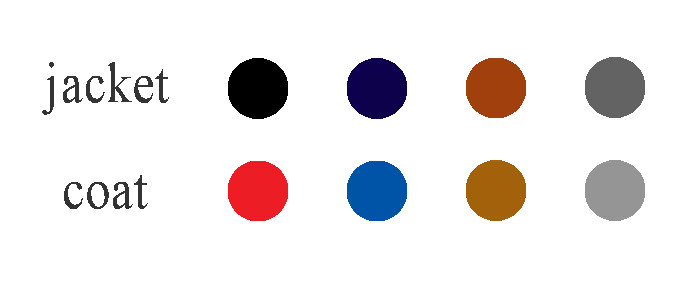
\includegraphics[page=1,width=\textwidth]{Figures/jacket_coat.pdf}
    \caption{How semantic similarity can be shown using similarity of two vectors, the colour gradient represents similar values for elements of the vector}%
    \label{fig:jacket_coat}
\end{figure}

% Count based approaches to predictive approaches
% Conventional VSM produces high dimensional representations, since the dims. correspond to words in the number can reach millions -> don't know where I got this, can't use it as it probably plagiarism
\subsection{Distributed Vector Representations}%
\label{sub:distributed_vector_representations}
% https://www.gavagai.se/blog/2015/09/30/a-brief-history-of-word-embeddings/
% Wish this post had an author, main takeaways;
% The main difference between these various models (neural language models and distributional semantic models) is the type of contextual information they use.
% LSA and topic models use documents as contexts, which is a legacy from their roots in information retrieval.
% Neural language models and distributional semantic models instead use words as contexts, which is arguably more natural from a linguistic and cognitive perspective.
% These different contextual representations capture different types of semantic similarity; the document-based models capture semantic relatedness (e.g. “boat” – “water”) while the word-based models capture semantic similarity (e.g. “boat” – “ship”).
% This very basic difference is too often misunderstood.

% \textcite{bengio_neural_2000} root word embedding paper.
% EVERYONE says they coined 'word embeddings', doesn't appear in the paper, don't know where people got that
% There is another paper called A Neural Probabilistic Language Model, that came out in 2000
% People pretend that it doesn't exist, we'll use the 2003 one as well, it's just the extended version I think

% So far we've been talking about IR, now this is language models
% For instance Turney Pantel (VSM Survey) doesn't mention bengio or any other word embeddings (2010)

% input layer -> emb. layer -> softmax layer
\textcite{bengio_neural_2003} proposed learning word representations using a feedforward neural network.
Their model learns feature vectors for words using a predictive approach instead of counting based approaches we have presented until now.
Although neural networks have been proposed to learn a language model by \textcite{xu_can_2000}, the main contribution of \citeauthor{bengio_neural_2003} is to use an \emph{embedding layer}, in order to attack \emph{curse of dimensionality}.
Their approach was also motivated exponentially increasing size of the vocabularies caused by \emph{n-grams}.
n-grams are representations that are built using multiple tokenized words.
For instance, as well as showing \emph{new} and \emph{york} in the vocabulary, \emph{New York} is handled as a single unit.
For a corpus with vocabulary $V$, there are $|V|$ dimensions for the language model to learn and taking \emph{n-gram} representations into consideration, the problem grows exponentially.
Using $m$ dimensions in the embedding layer allowed \citeauthor{bengio_neural_2003} to represent words using manageable, more representative dimensions and the problem scaled linearly as a result.

The setup for the neural network starts with the one hot encoded vector representation of the context for a word $w$, essentially a one dimensional vector where context words of $w$ are set while the rest of the vocabulary are zero.
This context window is similar to those used in statistical models that predicts the word $w_t$ using the words that lead up to $w_t$.
In other words, context window of $w_t$ is $T$ words on the left of $w_t$.
In the following equation, we present the problem algebraically with an arbitrary probability function $P$.

\begin{displaymath}
    P(w_1^T) = \prod_{t=1}^{T}P(w_t | w_{1}^{t-1})
\end{displaymath}

In short, the input layer is projected into an embedding layer, later to a softmax layer to get a probability distribution in order to minimize the following softmax cost function.

\begin{equation}%
    \label{eqn:bengio_softmax}
    \hat{P}(w_t|w_{t-1}, \dots, w_{t-n+1}) = \frac{e^{y_{w_{t}}}}{\sum_{i}e^{y_{i}}}
\end{equation}

However, this formulation is too computationally expensive since all vocabulary needs to be considered for the sum in the denominator.
The curse of dimensionality problem is shifted to the final layer of the neural network.
It will be solved later using hierarchical softmax~\cite{mikolov_distributed_2013}.
Authors reported training times around 3 weeks using 3 to 5 context window sizes and vocabulary sizes around 17000.

\textcite{collobert_unified_2008} suggested a deep neural network model in order to learn feature vectors for various natural language processing tasks.
Their proposed approach for language model is important for our case since it explicitly learned distributed word representations or simply \emph{word embeddings}.
They have introduced two key ideas;
\begin{itemize}
    \item Instead of using a context window that used words left of the target word to estimate the probability of the target word, they have placed the context window \emph{on} the target window, using $n$ words for left and right of the target word.
    \item They introduced negative examples, where they randomly changed the middle word with a random one. As well as keeping their model from overfitting, this allowed them to use the ranking cost;
        \begin{displaymath}
            \sum_{s \in S} \sum_{w \in D} \text{max}\big( 0, 1 - f(s) + f(s^w)\big)
        \end{displaymath}
\end{itemize}

% Turian 2010 doesn't appear much in any of the surveys or word embedding blogs
% but as far as I can tell, they're the first to say word embeddings are useful because they're off the shelf which I want to emphasize
% Like they literally say "With this contribution word embeddings can now be used off-the-shelf as word features, no tuning"

\subsection{Pre-trained Embeddings}%
\label{sub:pre_trained_embeddings}

\textcite{p._turian_word_2010} evaluated the performance of different word representations as word features that researchers can include into an existing task.
Their contribution is elegantly summarized in their work as;
\begin{displayquote}
    Word features can be learned in advance in an unsupervised, task-inspecific, and model-agnostic manner.
    These word features, once learned, are easily disseminated with other researchers, and easily integrated into existing supervised NLP systems. \\
    \textelp{} \\
    With this contribution, word embeddings can now be used off-the-shelf as word features, with no tuning.
\end{displayquote}

% Jointly with \citeauthor{collobert_unified_2008}, \citeauthor{p._turian_word_2010} steered the work on word representations to the today's route.
% They showcased that word embeddings can indeed be used as ready made feature vectors and once trained, can be used for other applications by other researchers.
% Important to note that they reported training times in the order of days, even weeks.

% \textcite{mikolov_distributed_2013} word2vec paper.
% This paper is legendary, talk about skip-gram, hierarchical softmax negative sampling
% Also this paper is cursed and I can't explain it to save my life.
% And the approaches are rabbit holes and I don't have time
% If need be, \cite{goldberg_word2vec_2014} -> word2vec explained

\subsection{Popularization of Word Embeddings}%
\label{sub:popularization_of_word_embeddings}

word2vec package~\cite{mikolov_efficient_2013,mikolov_distributed_2013,mikolov_linguistic_2013} popularized word embeddings.
There are two aspects of the work done by \citeauthor{mikolov_distributed_2013}  that contributed to the fact;
\begin{itemize}
    \item Their model captures the semantic and syntactic attributes of words and phrases on a large scale with good accuracy, trained on billions of words using a shallow neural network, keeping the computational cost down.
    \item They published their code as well as their pre-trained embeddings as an open source project\footnote{\url{https://code.google.com/archive/p/word2vec/}}.
\end{itemize}
The second point is self explanatory but in order to argue about the first one, we should report the algorithms behind word2vec.

The \emph{skip-gram model} introduced by \textcite{mikolov_efficient_2013} differs from the previous methods by predicting the surrounding words given the target word (Figure~\ref{fig:skipgram}).

\begin{figure}[htbp]
    \centering
    \incfig{skip_gram_2}
    \caption{Skipgram architecture by \textcite{mikolov_distributed_2013}}%
    \label{fig:skipgram}
\end{figure}

In \citetitle{mikolov_distributed_2013}, it is defined as follows;
\begin{equation}
    \frac{1}{T}\sum_{t=1}^{T}\sum_{-c \leq j \leq c, j \neq 0} \log p(w_{t+j}|w_t)
\end{equation}
%The $w_{t-c}, w_{t-c+1}, \dots, w_{t+c-1}, w_{t+c}$ are the context of the word $w_t$.
The $w_{1}, w_{2}, \dots, w_{T}$ are the context of the word $w_t$.
%It includes $c$ words behind and $c$ words ahead of the word $w_t$.
We should note that, \textcite{levy_improving_2015} has identified that this window size is \emph{dynamic} in the open source implementation of word2vec, where the actual window size is sampled between $1$ and $T$.

Following word2vec, \textcite{pennington_glove_2014} introduced GloVe embeddings that were built on word co-occurrence probabilities.

% In the Equation~\ref{eqn:bengio_softmax}, we have reported on the \emph{costly} softmax function, used by \citeauthor{bengio_neural_2003}.
% \citeauthor{mikolov_distributed_2013} significantly improves their model's performance by using \emph{hierarchical softmax}.
% Hierarchical softmax~\cite{morin_hierarchical_2005} uses a binary tree to distribute the probability distribution among the leaves of the nodes.

%The theory set out by ? was empirically shown by \citeauthor{mikolov_distributed_2013} by demonstrating that countries and their capital cities exhibited a linear pattern on the PCA.

% http://blog.aylien.com/overview-word-embeddings-history-word2vec-cbow-glove/
% Ruder says don't dwell on the specific embedding too much
% fasttext is trained on a huge corpus with tuned hyperparameters
% hence the choice of the specific model is not important
\textcite{levy_improving_2015} compared the performance of count based and prediction based word representation models.
Representation algorithms they considered are;
\begin{itemize}
    \item Positive pointwise mutual information (PPMI)~\cite{church_word_1990, bullinaria_extracting_2007}
    \item Singular Value Decomposition on PPMI Matrix (Latent Semantic Analysis)~\cite{deerwester_indexing_1990}
    \item Skip-Gram with Negative Sampling~\cite{mikolov_distributed_2013}
    \item Global Vectors for Word Representation~\cite{pennington_glove_2014}
\end{itemize}
They found out that choice of a particular algorithm played an insignificant role compared to choosing the right approach during training, mainly picking correct \emph{hyperparameters}.
Besides, the amount of data the models are trained on were more important than the model itself.
They used this finding to counter the results reported by \textcite{baroni_dont_2014}.
\citeauthor{baroni_dont_2014} claimed that predictive models outperformed count based models.
On the other hand, \citeauthor{levy_improving_2015} noted that \citeauthor{baroni_dont_2014} used count based models without hyperparameter tuning, denying them from \enquote{tricks} developed in the word representation literature.
Finally, \textcite{levy_neural_2014} emprically proved that word2vec's skip gram with negative sampling approach is equivalent to factorizing a word-context matrix weighted using positive pointwise mutual information.
With the amount of overlap and marginal performance gains in between the algorithms, the choice of a particular model seems not as important.

\subsection{fastText}%
\label{sub:fasttext}

%Finally, word2vec lead up to \textcite{bajo}
% bag of character n-grams, no need to worry about mophological structure of the language, can induce oov words if parts of it are available,
% Ruder survey demonstrated how good at compositing they are *citation needed*
Armed with the fact that a good word representation model should tune their hyperparameters and should be trained on a large dataset, we set our sights on \emph{fastText}.
On their website, authors define fastText as a \enquote{Library for efficient text classification and representation learning}.
The ideas behind it are presented in \textcite{mikolov2018advances}.
Overall, it builds upon word2vec~\cite{mikolov_distributed_2013} by adding position dependent features presented in \textcite{mnih_learning_2013} and character n-grams suggested on \textcite{bojanowski_enriching_2016}.

Let us turn our focus towards \citetitle{bojanowski_enriching_2016}~\cite{bojanowski_enriching_2016}.
Instead of using a context window to learn the representation of the target word or predicting surrounding words given the centre word like in the the skip-gram model, \citeauthor{bojanowski_enriching_2016} learn representations for character n-grams.
We have mentioned that n-grams consider sequences like \emph{New York} as a single token.
Character n-grams start with parsing the corpus into $c$ character long sequences.
We will use 3 as the $c$ value.
The boundaries of the words are marked with \enquote{<>} characters for later and the whole corpus is transformed into tokens where the phrase \enquote{lecture slide} is now \enquote{<lecture> <slide>}.
Then, sequences of 3 characters are extracted such that \enquote{<slide>} is broken down into \enquote{<sl, sli, lid, ide, de>}.
Note that \enquote{lid} character n-gram is different from word \enquote{<lid>}.
These character n-grams are called subword vectors, they are trained using the skip-gram architecture.

\begin{figure}[htbp]
    \centering
    \includegraphics[page=1,width=\textwidth]{Figures/fasttext.pdf}
    \caption{Overview of character n-gram model}%
    \label{fig:fasttext}
\end{figure}

With the subword vectors $z_g$ for every n-gram $g$ at hand, authors take a dictionary of n-grams of size G and for a given word $w$, they denote $G_{w} \subset {1, \dots, G}$ as the n-grams of $w$.
So the scoring function for the word in accordance to word's context n-grams is~\cite{bojanowski_enriching_2016};
\begin{displaymath}
    s(w,c) = \sum_{g \in G_{w}}z_{g}^T v_c
\end{displaymath}

\textcite{grave_learning_2018} trained fastText model on different languages using Wikipedia and Common Crawl data.
Wikipedia is a curated encyclopaedia that can be used as a multilingual corpora with 28 languages that have over \emph{100 million} tokens and 82 languages with 10 million tokens~\cite{grave_learning_2018}.
Considering the original word2vec was trained on \emph{100 billion} tokens, \citeauthor{grave_learning_2018} also used Common Crawl, a non profit project that collocates web pages and publishes the data publicly.
This data can be inadvertently noisy which \citeauthor{grave_learning_2018} addressed using linewise language identification and by removing duplicate lines that often appear as leftover boilerplate on many sites.
While Wikipedia provided them with a curated signal, Common Crawl data helped with capturing as many contexts as possible to train their distributed model.
They are currently hosting the pre-trained word embeddings on their website~\footnote{\url{https://fasttext.cc/}}.

\subsection{ConceptNet Numberbatch}%
\label{sub:conceptnet_numberbatch}

As an alternative to purely distributional models, \textcite{speer_conceptnet_2017} suggested \emph{numberbatch} embeddings built in conjugation with ConceptNet.\footnote{\url{http://conceptnet.io/}}.
ConceptNet is a knowledge graph.
Like the WordNet, it presents semantic relationships between concepts but the defined relationships are more fine grained.
The relationships are collocated from various resources like English Princeton WordNet, Open Mind Common Sense~\cite{anacleto_can_2006} and DBPedia~\cite{auer_dbpedia_2007}.
ConceptNet stylizes its relations with the \texttt{/r/Relationship} syntax.
For instance, being distinct members of a set relation is defined as \texttt{/r/DistinctFrom} which includes concepts like August and September.\footnote{\url{https://github.com/commonsense/conceptnet5/wiki/Relations}}.
Compared to WordNet, more subjective, human centric relations are defined such as \texttt{/r/MotivatedByGoal}, relationship between \emph{compete} and \emph{win} or \texttt{/r/ObstructedBy}, the relationship between \emph{sleep} and \emph{noise}.
Total number of relations that are available between two concepts is 36.
Moreover, these relationships are \emph{weighted} depending on how present they are.
For example, the concept \emph{run} is related to \emph{fast} with a weight of \texttt{9.42} but the similarity between \emph{race} and \emph{run} is weighted at \texttt{2.54}.
Finally, the ConcepNet is multilingual, encompassing 304 languages in total but only 10 languages have full support and advised to use for downstream applications.
For our case, only Italian is fully supported by numberbatch while the rest of the languages fall into the 77 languages which reported as having moderate support and may be used in downstream tasks with loss in performance.
Details of the knowledge graph and the procedure is explained by \textcite{speer_conceptnet_2017} in the paper \citetitle{speer_conceptnet_2017}.

\citeauthor{speer_conceptnet_2017} also present their resource in word embedding matrix form for ease of use in the current plug-and-play environment.
In order to get word embeddings from the knowledge graph, first they prepare a symmetric term-term matrix $X$ where an element $w_{i,j}$ is the sum of all edge weights between terms $i$ and $j$.
This is similar to a word co-occurrence matrix but instead of constructing the matrix using unstructured text, this approach builds upon semantic connections between senses.
\citeauthor{speer_conceptnet_2017} reports that their approach learns \emph{relatedness} more so than \emph{similarity} which was reported by the word co-occurrence approaches before~\cite{lund_producing_1996}.

With the term-term matrix at hand, \citeauthor{speer_conceptnet_2017} weigh the terms using positive pointwise mutual information (PPMI) as suggested by \textcite{levy_improving_2015} and reduce it to 300 dimensions, as is standard set by word2vec, using truncated SVD\@.
Resulting matrix is similar to approaches set by \textcite{deerwester_indexing_1990} or \textcite{pennington_glove_2014} but \citeauthor{speer_conceptnet_2017} enrich it further using \emph{retrofitting} as proposed by \textcite{faruqui_improving_2014}.
Pre-trained word2vec and GloVe embeddings are incorporated into the reduced term-term matrix to finally obtain embeddings that include both distributional and semantic relatedness signal.
Authors call their finalized model \emph{ConceptNet numberbatch}.
\citeauthor{speer_conceptnet_2017} reports state of the art results compared to word2vec embeddings on word relatedness and models built using their embeddings get scores equivalent to humans on SAT-style analogy tasks.

% \section{Bilingual Word Embeddings}%
% \label{sec:bilingual_word_embeddings}

% Cross lingual embedding models optimize similar objectives.
% Only source of variation is due to the data used and the monolingual regularization objectives employed~\cite{ruder_survey_2017}.

\section{Approaches in Wordnet Generation}%
\label{sec:approaches_in_wordnet_generation}

\subsection{History of Wordnet Generation}%
\label{sub:history_of_wordnet_generation}

We have mentioned the lexical database WordNet created by Princeton University.
To reiterate, WordNet is a lexical database with human annotated collection of senses and relationships among them.
The relationships are hierarchical so they can be followed along to reach new nodes due to the transitive property (shown in Figure~\ref{fig:hyponymy}).
The format itself has become the standard for databases that present meanings and concepts~\cite{neale_survey_2018}.

Glosses or the definitions that go along with synsets were not initially part of the WordNet design.
Authors believed that \enquote{definition by synonymity} would be enough.
In other words, definition of a synset can be derived from the lemmas that make up the synset.
As the number of items in the WordNet grew, only then short glosses, later followed by longer definitions got included in WordNet~\cite{fellbaum_wordnet_1998}.

\begin{table}[htbp]
    \centering
    \begin{tabulary}{\textwidth}{LL}
        \toprule%
        \textbf{Synset} & \textbf{Gloss} \\
        \midrule%
        \{glossary, gloss\} & an alphabetical list of technical terms in some specialized field of knowledge; usually published as an appendix to a text on that field \\
        \cmidrule(rl){1-2}
        \{dog, domestic dog, Canis familiaris\} & (a member of the genus Canis (probably descended from the common wolf) that has been domesticated by man since prehistoric times; occurs in many breeds) \\
        \cmidrule(rl){1-2}
        \{university\} & (the body of faculty and students at a university) \\
        \cmidrule(rl){1-2}
        \{depository financial institution, bank, banking concern, banking company\} & (a financial institution that accepts deposits and channels the money into lending activities) \\
        \bottomrule %
    \end{tabulary}
    \caption{Example synsets and their respective glosses}%
    \label{tab:synset_gloss}%
\end{table}

WordNet has been used in various natural language processing applications over the years such as text summarization~\cite{ercan_using_2007} or word sense disambiguation~\cite{banerjee_adapted_2002}.
Since the original WordNet was prepared for English over many years of work, efforts for creating an equivalent resource for other languages has been initiated.
Arguably, EuroWordNet set the standard for creating wordnets for languages other than English~\cite{vossen_introduction_1998, vossen_eurowordnet_2004}.

EuroWordNet\footnote{\url{http://projects.illc.uva.nl/EuroWordNet/}} project was initiated to introduce the benefits of English Princeton WordNet for other languages.
Additionally, an interlinked semantic network can be a research topic on lexicalization patterns of languages, finding conceptual clusters of vocabularies or cross lingual text retrieval~\cite{gonzalo_applying_1998, vossen_introduction_1998}.
EuroWordNet project included 7 wordnets for languages other than English and an adapted English wordnet.
Due to the effort needed to create a wordnet from scratch, \citeauthor{vossen_introduction_1998} averted the EuroWordNet project from creating full scale semantic lexicons and prioritized the connectivity between wordnets.
All in all, \textcite{vossen_introduction_1998} defines the aims as;
\begin{displayquote}
    \begin{enumerate}
        \item to create a multilingual database;
        \item to maintain language-specific relations in the wordnets;
        \item to achieve maximal compatibility across the different resources;
        \item to build the wordnets relatively independently (re)-using existing resources;
    \end{enumerate}
\end{displayquote}

One challenge in achieving compatibility is the shortcomings of using the original WordNet as the anchor.
On one hand, since the WordNet is the first and the most comprehensive, it is a natural hub for new wordnets.
On the other hand, a sense in one language might not have a direct equivalent in an other.
Cultural differences or linguistic differences between languages contribute to this fact~\cite{kitamura_cultural_2009} which is called a lexical gap or untranslatability.
EuroWordNet addresses lexical gaps using Inter-Lingual-Index (ILI).
ILI is a higher order list of meanings just for wordnet synsets to align themselves to, elevating the burden for alignment from English Princeton WordNet.
The introduction of ILI allowed language specific structures to exist in wordnets while keeping the connections among themselves.

% \begin{enumerate}
% \item Expand model, \textcite{vossen_introduction_1998}, fixed synsets are translated from English to target language.
% \item Link English entries from machine-readable bilingual dictionaries to English Princeton WordNet senses~\textcite{knight_building_1994}.
% \end{enumerate}
Two approaches for wordnet generation were defined by \citetitle{vossen_introduction_1998};
\begin{description}
    \item[Merge Approach] where a wordnet structure is formed in the target language with synset selection and relation mapping. Then the connections between the new wordnet and English Princeton WordNet can be established.
    \item[Expand Approach] where English Princeton WordNet is (machine) translated to target language~\cite{knight_building_1994}, preserving connection information with a trade-off where the target language wordnet will be biased towards the relationships of the English Princeton WordNet and may not include target language specific lexical connections.
\end{description}

In order to maintain as much language specific lexical connections as possible while having a starting point for evaluation of target wordnets, EuroWordNet project offered \enquote{Base Concepts}.
This idea evolved into 1000 and later to 5000 core synsets that are compiled from most frequent, connected and representetive synsets to be used for evaluating wordnet generation~\cite{boyd-graber_adding_2006}.

\subsection{Examples of Wordnet Generation}%
\label{sub:examples_of_wordnet_generation}

Following the EuroWordNet project, several studies were published on wordnet generation with proposals heavily leaning towards the expand approach.
\textcite{diab_feasibility_2004} explored whether an Arabic wordnet is attainable or not using a parallel corpora.
Arabic differs from the languages explored in EurowordNet due to its unusual morphological nature.
Using their proposed method, they observed 52.3\% of words they processed are sufficient for a future Arabic wordnet.
They have also reiterated that semantic relationships in a language are transferable to a target language's wordnet.

% \textcite{ruiz-casado_automatic_2005} explored using online encyclopaedia Wikipedia to automatically discover potential synsets using the definitions in the term's pages.
% Just English
Further approaches using parallel corpora to align the target language with English Princeton WordNet were used by \textcite{sagot_building_2008} in order to create a production ready French wordnet and by \textcite{fiser_leveraging_2009} to create a Slovene wordnet.

Approaches that used machine translation to get potential synsets for the target language was explored by \textcite{lam_automatically_2014}.
They proposed two approaches for this task.
First approach uses a single bilingual dictionary to translate English Princeton WordNet lemmas to target language to form synsets.
Second approach translates existing wordnet synsets to English and then translates them to target language.

Following the publication of word2vec, approaches that use word embeddings gained traction and are interest to us.
\textcite{sand_wordnet_2017} used word embeddings to extend Norwegian wordnet by adding new relationships on existing synsets or by introducing new synsets all together.
First, cosine similarity measure is used to discover nearest neighbours to a potential synset.
Then a threshold value is used to cut off any new synsets below a certain similarity value.
They evaluated their approach against accuracy, the percentage of relations that were correct and attachment which is similar to a recall score.
It is the percentage of considered synsets that were above the threshold value.
Overall, \citeauthor{sand_wordnet_2017} reported accuracy scores within the 55.80 to 64.47 percent range with respect to different frequency thresholds and an attachment score that fluctuate between 96.20 and 98.36 percent.

%\textcite{khodak_automated_2017} used word embeddings and WordNet.
% talk about Khodak -> Automated WordNet construction Using Word Embeddings
Arguably most relevant to our study, \textcite{khodak_automated_2017} proposed an unsupervised method for automated construction of wordnets.
In their paper \citetitle{khodak_automated_2017} they present 3 approaches and compare their precision, recall and coverage.

First off, they picked 200 French and Russian adjectives, nouns and verbs, totalling 2 corpora with 600 items in each.
These words are selected based on if they have a translation in the core sense list provided by English Princeton WordNet.
Their approach starts with the processing of a word $w$.
Initially, the presented method collects the possible translations of $w$ using a bilingual dictionary and uses them as lemmas to query English Princeton WordNet.
As we have mentioned, lemmas that query the WordNet retrieve synsets in the form \texttt{<lemma.pos.offset>}.
Furthermore, every synset includes possible lemmas that can represent the sense of the synset (Refer to Table~\ref{tab:synset_gloss}).
These lemmas form the set $S$.
By translating the English Princeton WordNet lemmas to target language, they obtain the set $T_S$
Elements of $T_S$ and $w$ are both in target language so a monolingual word embeddings can be used;
As a baseline, they calculate the average cosine similarity between word embeddings of every element of $S$ and $w$.

\begin{displaymath}
    \frac{1}{S}\sum_{w' \in S}v_{w} \cdot v_{w'}
\end{displaymath}

In order to improve the discriminative power of their target vectors, they use synsets relations, definitions and example sentences.
These are used to get a more representative vector $v_{L}$.
Given resources can be thought as sentences and sentence embeddings are calculated by getting a weighted average of word vectors of words that make up the sentence.
The weighting is called smooth inverse frequency which was suggested by \textcite{arora_simple_2016};

\begin{displaymath}
    v_{L} = \sum_{w' \in L}\frac{a}{a + P{w'}}v_{w'}
\end{displaymath}

We will talk about sentence embeddings in detail for our approach in Section~\ref{sec:linear_assignment_using_sentence_embeddings}.

\section{Other Related Work}%
\label{sec:other_related_work}

\textcite{lesk_automatic_1986} presented the \emph{Lesk Algorithm} which is one of the earliest answers to word sense disambiguation problem.
This classic algorithm identifies the correct sense for a couple of words among their synonyms using the word that it co-occurs with.
The classic example uses the \emph{pine cone} for demonstration.
First, the dictionary definitions of the two words in the sentence are extracted.
For \emph{pine}, the definitions are \enquote{kind of evergreen tree with needle-shaped leaves \dots} and \enquote{waste away through sorrow or illness \dots}.
For \emph{cone}, the definitions are presented as \enquote{solid body which narrows to a point \dots}, \enquote{something of this shape whiter solid or hollow \dots} and \enquote{fruit of certain evergreen trees}~\cite{lesk_automatic_1986}.
The algorithm then assigns the sense pairs that have the highest number of word overlaps between them.
For the \emph{pine cone} case, the algorithm finds the overlap on \emph{evergreen} and \emph{tree} to assign the matching senses; \enquote{kind of evergreen tree with needle-shaped leaves \dots} and \enquote{fruit of certain evergreen trees}.
This approach relied on the definitions given by traditional dictionaries.

\textcite{banerjee_adapted_2002} extended the \emph{Lesk Algorithm} by levering the WordNet synsets.
Instead of comparing the definitions of the pair of words, their approach uses the definitions of the co-occurring words as well as the definitions of synsets that are connected to the word pair.

\textcite{gordeev_unsupervised_2018} presented various approaches for matching cross lingual product classifications or product taxonomies using bilingual embeddings.
Their work is highly related since they have also studied the viability of showing senses using word embeddings on a latent space which were Russian and English product descriptions.
However, they relied on other information sources such as the category of the products which is absent in our study.
Our study and their approaches are similar in an additional way; they reported some products did not have direct equivalents on the target language's product space, which highly resembles the lexical gap we have talked about in Section~\ref{sec:approaches_in_wordnet_generation}.
They also used out of domain pre-trained word embeddings due to small size of their corpora.

Three algorithms that were presented which are relevant to our study;
\begin{enumerate}
    \item doc2vec~\cite{le_distributed_2014} on untranslated text.
    \item doc2vec on translated text.
    \item averaging the category description vector.
\end{enumerate}
\citeauthor{gordeev_unsupervised_2018} reported 19.75\% accuracy on the first approach and 44\% on the second approach.
Like our case, their best results came from using out of domain word embedding vectors to encode the text at hand, which is presented in the third approach with an accuracy of 55\%.
